\section{Hyper-Converged Infrastructure (HCI)} \label{section: HCI}

HCI, or Hyper-Converged Infrastructure, is a software-defined, unified system that combines the traditional elements of IT infrastructure (e.g., compute, networking, management, storage) with virtualization, simplifying infrastructure, reducing costs, and increasing scalability and flexibility. In a traditional IT Infrastructure, servers, storage networks, and storage systems are physically separated as stand alone hardware devices (e.g., servers, network switches, disk arrays). Consolidating these components into a single, integrated system simplifies the management, deployment, configuration, and maintenance of your IT Infrastructure. 

The benefits of an HCI environment include: 
\begin{itemize}
    \item Scalability: Designed to scale out by adding additional nodes on-demand to your system.
    \item Efficiency: Improve resource utilization by using or eliminating idle storage capacity.
    \item Agility: Quickly deploy new applications and workloads without extensive planning across systems. 
    \item Data Protection: Integrated backup and disaster recovery.
    \item Reduced Hardware Costs: Reduce the amount of hardware required reducing CAPEX\footnote{Capital expenditure is the cost a business incurs to acquire assets that will provide benefits beyond the current year.}/OPEX\footnote{Operating expenses refer to the money a company spends to run day-to-day operations.} costs. 
\end{itemize}

% Single-Machine HCI Relationship with Cloud Deployments %
%\begin{figure}[H]
%    \centering
%    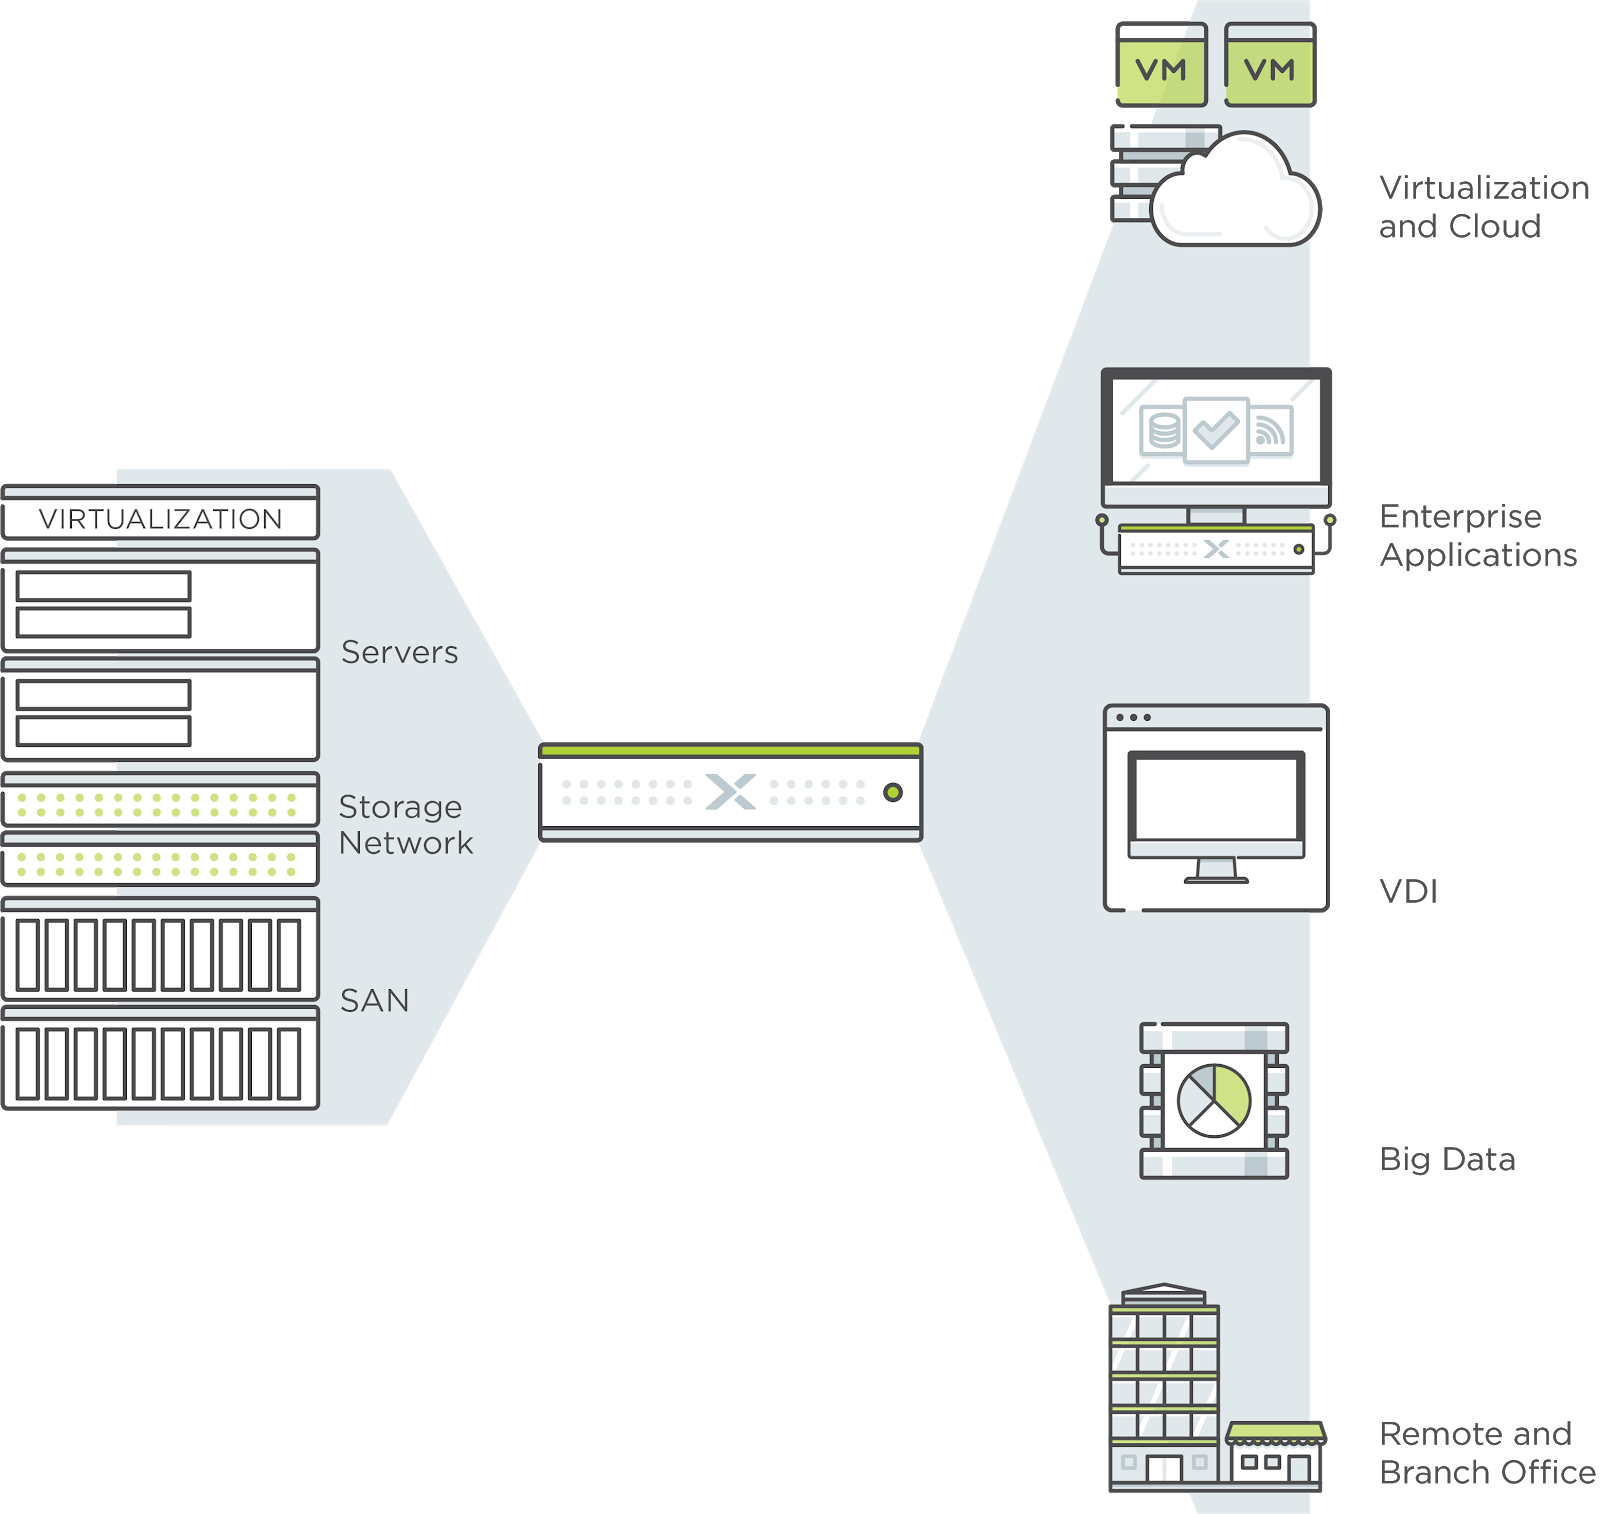
\includegraphics[scale = 0.25]{images/HCI_Nutanix_Node.png}
%    \caption{Single-Machine HCI \textcolor{red}{(STOLEN EXAMPLE)}}
%    \label{HCI Explained (Single-Machine)}
%\end{figure}

\begin{figure}[H]
    \centering
    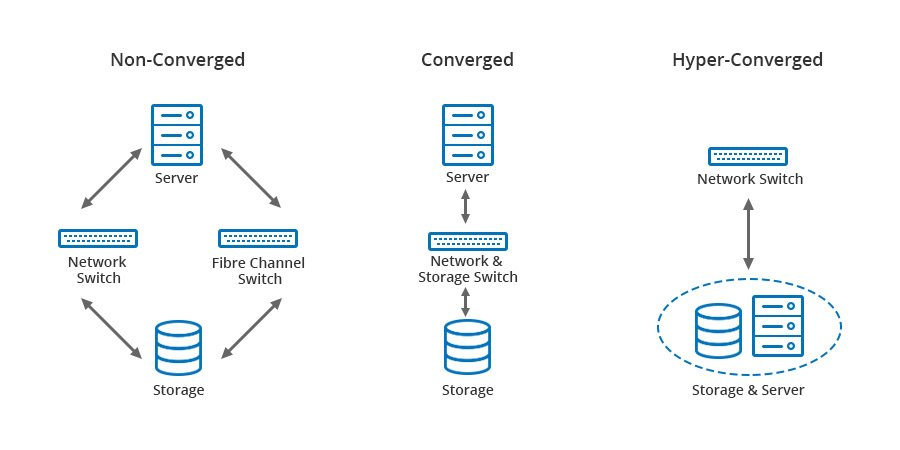
\includegraphics[scale = 0.5]{images/HCI_tldr.jpg}
    \caption{Types of IT Infrastructures \textcolor{red}{(STOLEN EXAMPLE)}}
    \label{HCI Convergance Comparison}
\end{figure}

In HCI, multiple servers or nodes are combined to create a cluster. These nodes share their computing and storage resources with each other to create a multi-purpose integrated system. The design of your HCI cluster will depend on your specific needs and requirements.

The software that powers HCI also includes a management layer, which automates tasks like resource provisioning, data migration, and load balancing. This layer abstracts the hardware, making it easier to manage and deploy your IT infrastructure. Overall, HCI is a powerful and flexible solution that can help organizations streamline their IT operations, reduce costs, and improve efficiency.
